\selectlanguage{portuguese}
\section{Introducción}
\label{sec:introduccion}

La construcción de una línea de transporte de electricidad requiere
bastante preocupación. Es muy importante construirla en la forma que
reduce al mínimo el riesgo de dañar a personas. Hay que asegurarse que
la línea está a una distancia suficiente del suelo, edificios y que la
construccion es estable. Además, ciertos factores deben ser
considerados, por ejemplo, la longitud del cable eléctrico producido
por el tiempo, la temperatura del ambiente o las velocidades máximas
de vientos que se registran y que puedan producir deterioro o rotura del
cable.

%\begin{mybox} 
%  \vspace{-21pt}
\begin{figurebox}
  \vspace{20pt}
  \centering
  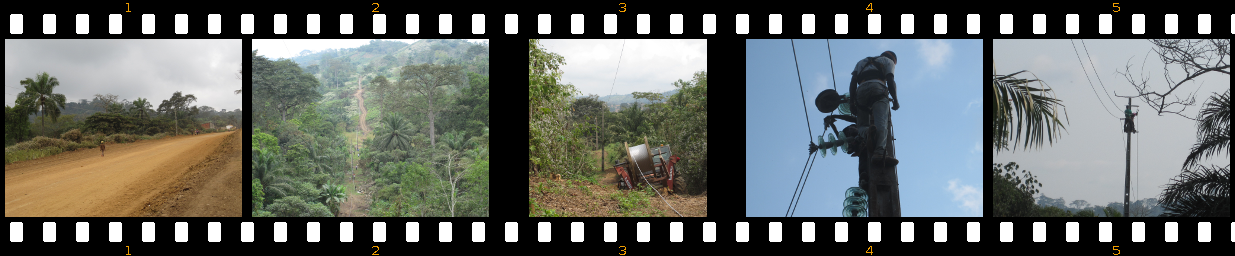
\includegraphics[scale=0.35]{InstalacionLinea.png}\\
  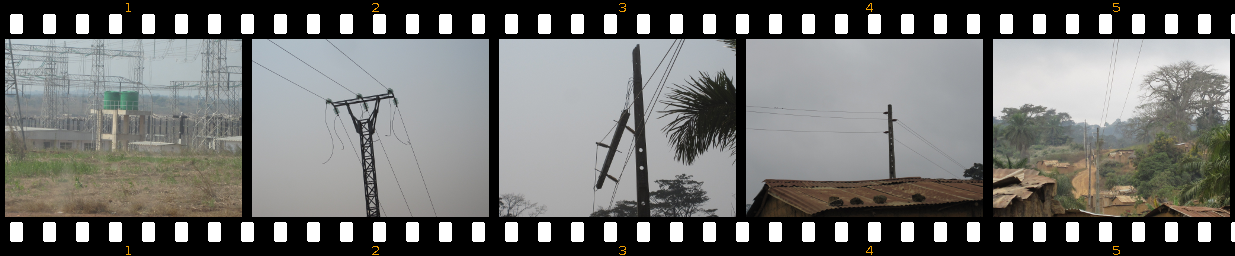
\includegraphics[scale=0.35]{InstalacionLinea2.png}\\
  Imágenes de una instalación eléctrica en Ángola\\ 
\end{figurebox}
% \vspace{-20pt}
%\end{mybox}

Y es aquí donde la Matemática y la Física entran en acción. Con su
ayuda podemos construir una línea eléctrica que no solo es segura sino
que también puede optimizarse el valor del coste de de la
construcción. Años de experiencia de ingenieros de todo el mundo
muestran claramente que las matemáticas y la física no se equivocan y
existen diferentes modelos que cumplen distintas normativas que
garantizan seguridad.  En Ángola existe un reglamento de seguridad de
construccion de líneas eléctricas de alta tensión y que puedes
encontrar en nuestro formato online de la revista en la pestaña de
\emph{Documentacion} y será el que consideramos en este artículo para
realizar algunos cálculos mecánicos.

En la práctica, existen diferentes softwares, que permite diseñar las
líneas eléctricas y que ya tiene preprogramado las normativas del
lugar específico donde se quiere construir.  Aún cuando existen estos
programas el ingeniero que realiza el diseño con ellos debe conocer el
funcionamiento interno y ser capaz de interpretan los resultados del
programa y ver si son consistentes. Además el ingeniero, debe ser
consciente de la normativa del lugar donde va a construir y ver las
compatibilidades o incompatibilidades de la normativa que internamente
tiene el programa a utilizar.

En este artículo vamos a ver como la longitud del cable electrico de
una instalación eléctrica varía por la tensión de su propio peso, por
el viento y por la temperatura atmosférica.


\section{El concepto \emph{flecha}  de la catenaria}
\label{sec:parabola-vs-catenara}

En el número de enero de este año, estudiamos con profundidad la curva
de la catenaria y vimos que es la curva que describe, por ejemplo, un
cable eléctrico suspendido en dos postes. En esta sección vamos a
presentar lo que es la \emph{flecha} asociada a una catenaria y
presentar sus fórmulas. Este concepto es muy importante a tener en
cuenta en la construcción de líneas energéticas y la clave para la
seguridad de las personas.

\begin{wrapfigure}{r}{0.5\textwidth}
  \vspace{-.8cm}
  \begin{figurebox}
    \centering
    \begin{tikzpicture}
      \draw [bluesol] (0,0) -- (6,0);
      \draw [bluesol] (3,0) -- (3,5);
      \draw[domain=-3:3,smooth,variable=\x,redsol]
      plot({\x+3},{(exp(0.5*\x)+exp(-0.5*\x))});
      \draw[dashed] (0,2) -- (3,2);
      \draw[dashed] (0,0) -- (0,-1);
      \draw[dashed] (3,0) -- (3,-0.5);
      \draw[dashed] (6,0) -- (6,-1);
      \draw [<->,thick] (0,0) -- (0,2)
      node[midway,  rotate=90, yshift=-3mm] {{\tiny $a=\frac{T_v}{g\lambda}$}};

      \fill[bluesol] ( 0,4.7048) circle (0.1);
      \draw (-0.2,4.7048) node {$I$};

      \fill[bluesol] ( 6,4.7048) circle (0.1);
      \draw (6.3,4.7048) node {$S$};

      \draw[dashed] (0,4.7048) -- (6,4.7048);
      \draw [<->, thick,blue] (3,2) -- (3,4.7048)
      node[midway,  rotate=90, yshift=-3mm] {$f$ (flecha)};
      \draw [<->, thick] (0,-0.5) -- (3,-0.5)
      node[midway, yshift=-2mm] {$v/2$};
      \draw [<->, thick] (0,-1) -- (6,-1)
      node[midway, yshift=-2mm] {$v$ (vano)};
      \draw [<->, thick] (6,0) -- (6,4.7048)
      node[midway,  rotate=90, yshift=-3mm]{$a\cosh(v/(2a))$};

      % \draw[red] (6,4.25) .. controls (5.833,2) .. (3,2);
      % \draw[<->]  (6,4) .. controls (5.8,3) and (4.1,1) .. (3,1);

    \end{tikzpicture}
    \caption{El gráfico de la función $y =
      a\cosh(x/a)$.}
    \label{fig:1}
  \end{figurebox}
  \vspace{-.8cm}
\end{wrapfigure}

La \emph{flecha} de una catenaria es la máxima distancia desde la
linea que conecta los puntos de suspensión del cable hacia el
cable. Vamos a darle forma matemática a la  \emph{flecha} asociada a la
catenaria. La fórmula general de la catenaria es la siguiente:
\begin{equation}\label{cat:a}
  y = a\cosh\Big(\frac{x-C_1}{a}\Big)+C_2.
\end{equation}
Observa que las constantes $C_1$ y $C_2$ son constantes de translación en el eje $x$ y
en el eje $y$ respectivamente y por ello podemos considerar el caso cuando $C_1=C_2=0$. Así la Ecuación \ref{cat:a} la
reducimos a la siguiente,
\begin{equation}\label{cat:b}
  y = a\cosh\Big(\frac{x}{a}\Big),
\end{equation}
que depende del parámetro $a$ que es igual $\frac{T_0}{g\cdot\lambda}$ donde:
\begin{itemize}[noitemsep,nolistsep]
\item[$T_0$] es el valor de la componente horizontal de la tension (es
  constante en cada punto del cable, sus unidades son Newtons [\si{N}]),
\item[$g$] es la aceleración debida a la gravitación,
\item[$\lambda$] es el valor del peso del cable dividido por su longitud.
\end{itemize}


\begin{wrapfigure}{r}{0.5\textwidth}
  \vspace{-2.1cm}
  \begin{mybox}
    \centering
    \emph{\textcolor{bluesol}{Series de Taylor de cosenos y senos
        hiperbólicos.}}
    \begin{equation}
      \label{eq:10}
      \cosh(x)=1+\frac{x^2}{2!}+\frac{x^4}{4!}+\ldots,
    \end{equation}
    \begin{equation}
      \label{eq:11}
      \senh(x)=x+\frac{x^3}{3!}+\frac{x^5}{5!}+\ldots.
    \end{equation}
  \end{mybox}
  \vspace{-.8cm}
\end{wrapfigure}



%% Las unidades de la tensión son Newtons, pero en la práctica en
%% ingeniería es mucho más común utilizar kilogramos--fuerza, también
%% denominado \emph{kilopondio} ($[kgf]$).



Sustituyendo el valor de $a$, tenemos que la catenaria se escribe como
\begin{equation}\label{cat:c}
  y = \frac{T_0}{g \lambda}\cosh \left(\frac{x\cdot g \lambda}{T_0} \right).
\end{equation}
% y si reescribimos por $T_v$ a la constante $\frac{T_0}{g}$ nos queda
% \begin{equation}\label{cat:d}
%   y = \frac{T_v}{\lambda}\cosh\Big(\frac{\lambda}{T_v}x \Big).
% \end{equation}

Vamos a representar la ecuación de la catenaria escrita como en la
Ecuación (\ref{cat:c}) en la Figura \ref{fig:1} en rojo. En esta figura
podemos marcar en azul la distacia \emph{flecha} y llamamos \emph{vano} a la
distancia entre los postes de sujección de la catenaria y que representamos con $v$. De este modo
y observando la gráfica es muy fácil darle fórmula a la \emph{flecha}
que denotaremos por $f$:
\begin{equation}
  \label{eq:4}
  f =  a\cosh\Big(\frac{v}{2a}\Big)-a=
  \frac{T_0}{g\lambda}\Big(\cosh\Big(\frac{g\lambda v}{2T_0}\Big)-1\Big).
\end{equation}

Si queremos trabajar con calculadora podemos aproximar la flecha por
expresiones polinómicas usando aproximaciones de Taylor (véase
(\ref{eq:10})) de orden cuadrático por ejemplo, de la función coseno
hiperbólica. De este modo $f$ se puede aproximar por la siguiente
expresión:
 \begin{equation}
  \label{eq:12}
  f \approx{} \frac{v^2}{8a} = \frac{g\lambda v^2}{8T_0}.
\end{equation}

De este modo, conocer la \emph{flecha} nos permite tener controlado
distancias seguras. El problema viene cuando introducimos cambios de
temperatura, viento o el aumento de elasticidad del cable producido por el
tiempo. En las próximas secciones nos ocuparemos de los cambios de
longitud del cable por las anteriores razones y que deben tenerse
en cuenta a la hora de realizar una instalación eléctrica segura.

Finalmente, en esta sección vamos a calcular la \emph{longitud de un
  segmento de catenaria} medido desde el punto más bajo hacia el punto
al lado de la derecha que corresponde a la coordenada digamos $x$ y
que denotamos por $l(x)$. Esta longitud puede ser calculada usando la
fórmula que se demostró en el artículo de la catenaria de enero de
este año dado por la Ecuación (3.3) quedando,
\begin{equation}
  \label{eq:3}
  l(x) = a\senh(x/a)=\frac{T_0}{g\cdot\lambda}\senh\Big(\frac{g\cdot\lambda}{T_0}x\Big).
\end{equation}
Otra vez, aproximando por la Serie de Taylor (vea (\ref{eq:11})),
tenemos que
\begin{equation}
  \label{eq:14}
  l(x) \approx{} x+\frac{x^3}{6a^2}=x+\frac{(g\cdot\lambda)^2}{6T_0^2}x^3.
\end{equation}
Por lo tanto el longitud del cable es
\begin{equation}
  \label{eq:15}
  L = 2a\senh\Big(\frac{v}{2a}\Big)\approx{} v + \frac{v^3}{24a^2} = v
  + \frac{v^3(g\cdot\lambda)^2}{24T_0^2}.
\end{equation}

\section{Longitud del cable por la tensión}
\label{sec:cable-y-la}

\begin{wrapfigure}{r}{0.5\textwidth}
  \vspace{-1.5cm}
  \begin{mybox}
    \centering
    \emph{\textcolor{bluesol}{Datos mecánicos del cable LA-56}}
    
    \vspace{0.2cm}
    \begin{tabular}{llr}
      \toprule
      &Valor&Unidades\\
      \midrule
      Diámetro & 9,5 & [\si{mm}]\\
      Peso & 0,189& [\si{kgf}]\\
      Sección & 54,60 & [\si{mm^2}]\\
      Coeficiente de dilatación & 0,00001910 & \\
      Modulo elasticidad & 8100,00 & [\si{kgf/mm^2}]\\
      Carga rotura & 1670,00 & [\si{kgf}]\\
      \bottomrule
    \end{tabular}
  \end{mybox}
  \vspace{-1cm}
\end{wrapfigure}

Un problema que aparece cuando se colocan los cables eléctricos es que
estos se alargan si se les aplica una tensión. El parámetro que
corresponde a la elongación del cable es el módulo de la
elasticidad. Este parámetro, por ejemplo para un cable tipo LA-56 es
igual a 8100 kilogramos de fuerza por un milímetro cuadrado, esto es,
que un metro de cable se alarga $1/(8100\cdot 54.6)\approx 0.002$
milimetros si aplicamos un kilo de fuerza (un kilo de fuerza es igual
aproximadamente a \SI{9.81}{N}). En la Tabla se presenta
un ejemplo de los datos mecánicos del cable tipo LA-56 que es un tipo de cable que se suele
usar comunmente en las instalaciones eléctricas. La fórmula del \emph{alargamiento unitario} $\varepsilon$ es
$\varepsilon=F/(A\cdot E)$, donde $E$ es \emph{el módulo elastisidad}
también llamado \emph{el modulo de Young}, $F$ la fuerza, y $A$ la
sección del cable.



\begin{wrapfigure}{l}{0.5\textwidth}
  \vspace{-0.7cm}
  \begin{figurebox}
    \centering
    \begin{tikzpicture}
      \draw[->, very thick] (0,0) -- (6,0);
      \draw (3,-0.4) node {$T_0$};
      \draw [->, very thick] (0,0) -- (0,2);
    \draw (-0.4,1) node {$F_x$};
    \draw [->, very thick, bluesol] (0,0) -- (6,2);
    \draw [bluesol] (4.5,0.8) node {$T_x=\sqrt{T_0^2+F_x^2}$};
    \draw (0,-0.4) node {$P=(x,y)$};
    \draw [dotted, graysol] (0,2) -- (6,2);
    \draw [dotted, graysol] (6,0) -- (6,2);
    \draw [redsol, thick] (0,0) .. controls (2,0.8) and (2.5 , 1.2) .. (4,2.5);
    \draw [graysol, very  thick] (3,0) arc (0:18.435:3);
    \draw (2,0.3) node {$\alpha$};
      \draw [fill=black] (0,0) circle (0.1 );
    \end{tikzpicture}
    \caption{La tensión en el punto $x$}.
    \label{fig:5}
  \end{figurebox}
   \vspace{-1cm}
\end{wrapfigure}


Entonces, cuando colocamos el cable en los postes, este comienza a
sentir tensión. ¿Cuál es esta tensión? Mostramos una ilustración de
esta tensión en un punto $(x,y)$ del cable en la
Figura~\ref{fig:5}. Esta tensión, que llamamos $T_x$ está cuantificada
como sigue:
\begin{displaymath}
  T_x=\sqrt{T_0^2+F_x^2}
\end{displaymath}
y en la práctica se puede aproximar simplemente a su componente horizontal $T_0$.

Así, si suponemos  tenemos un cable tipo LA-56 que vamos a colgar entre
dos postes y su longitud antes de colgar era $L$ y la tensión medida
despues de colgar es $T_1$,  entonces su longitud $L_1$ después de colgar el cable es
\begin{displaymath}
  L_1 = L(1+\varepsilon)=L\left(1+\frac{T_1}{AE}\right),
\end{displaymath}
cuyas unidades son \si{kgf\per mm^2}.
%  y si reescribimos $t_1=T_1/A$ la anterior fórmula se simplifica como sigue:
% \begin{displaymath}
%   L_1=L(1+t_1/E)\textrm{, donde }t_1=T_1/A.
% \end{displaymath}
Entonces, si después, una fuerza exterior como el viento cambia la tensión
de cable a $T_2$, el cambio de longitud puede expresarse como sigue
\begin{equation}
 \label{eq:20}
 L_2-L_1=L\frac{T_2-T_1}{A\cdot E}.
\end{equation}

\section{Longitud del cable por la temperatura}

la temperatura atmosférica es otra condición climática que puede cambiar la longitud del cable. Si el cable en la temperatura de \SI{20}{\degreeCelsius}
tiene una longitud $L$, en la temperatura $\theta$ su longitud denotada por $L_{\theta}$ es
\begin{displaymath}
  L_{\theta}=L\cdot\alpha\cdot\theta,
\end{displaymath}
donde $\alpha$ es coeficiente de dilatación. Entonces la diferencia de longitud debido al cambio de temperatura entre una temperatura $\theta_1$ y $\theta_2$ es:
\begin{displaymath}
  L_{\theta_2}-L_{\theta_1} = L\cdot\alpha\cdot(\theta_2-\theta_1).
\end{displaymath}
Si añadimos este cambio de longitud de temperatura al cambio por la tensión del cable de la Ecuacion \eqref{eq:20} tenemos que,
\begin{displaymath}
  L_2-L_1 = L\cdot\alpha\cdot(\theta_2-\theta_1)-L\frac{T_2-T_1}{AE}.
\end{displaymath}
Utlizando \eqref{eq:15} por otro lado obtenemos que
\begin{equation}
  \label{eq:21}
  L_2-L_1=\frac{v^3g^2}{24}\Big(\frac{\lambda_2^2}{T_2^2}-\frac{\lambda_1^2}{T_1^2}\Big).
\end{equation}
Entonces,
\begin{displaymath}
  L\cdot\alpha\cdot(\theta_2-\theta_1)-L\frac{T_2-T_1}{AE}=\frac{v^3g^2}{24}\Big(\frac{\lambda_2^2}{T_2^2}-\frac{\lambda_1^2}{T_1^2}\Big),
\end{displaymath}
y si supnemos que $L\approx{}v$ entonces tenemos
\begin{equation}
  \label{eq:7}
  \alpha(\theta_2-\theta_1)-\frac{T_2-T_1}{AE}
  =\frac{v^2g^2}{24}\Big(\frac{\lambda_2^2}{T_2^2}-\frac{\lambda_1^2}{T_1^2}\Big).
\end{equation}



Un fuerte viento puede causar rotura del cable. Por esto en el cálculo
mecánico de una línea eléctrica hay que considerar este factor y
podemos ver esto reflejado en el ``Regulamento de segurança de linhas
eléctricas de alta tensão'' que impone las condiciones que la línea
tiene que
aguantar. Por ejemplo veamos los dos siguientes fragmentos de dos artículos:\\
{\bf Artigo 20º Hipóteses de cálculo:} ``Os condutores nus das linhas
devem ser calculados para a mais desfavorável das hipóteses
seguintes:''
\begin{itemize}[noitemsep,nolistsep]
\item[a)] na Zona Litoral Norte:
  \begin{itemize}[noitemsep,nolistsep]
  \item Temperatura de + 25° C e vento máximo habitual;
  \item Temperatura de +10° C e vento reduzido; 
  \end{itemize}
\item[b)] na Zona Litoral Sul:
  \begin{itemize}[noitemsep,nolistsep]
  \item Temperatura de + 25° C e vento máximo habitual;
  \item Temperatura de +5° C e vento reduzido; 
  \end{itemize}
\item[c)] na Zona Interior:
  \begin{itemize}[noitemsep,nolistsep]
  \item Temperatura de + 20° C e vento máximo habitual;
  \item Temperatura de 0° C e vento reduzido; 
  \end{itemize}
\end{itemize}
{\bf Artigo 23º Tensões máximas de tracção:} ``As tensões máximas de
tracção admissíveis para os condutores nus e para os tensores das
linhas não devem, para a hipótese de cálculo mais desfavorável
considerada no artigo 20º, ser superiores ao quociente das suas
tensões de rotura por 2,5.''

En otros paises, como por ejemplo Estados Unidos o  España hay
otro factor que hay que consider como el hielo que durante el
invierno se acumula encima del cable. Pero este tipo de situación no
suele ocurrir en Ángola y no la estudiamos en este artículo.

\section{Sobrecarga de viento}
\begin{wrapfigure}{r}{0.5\textwidth}
  \vspace{-1.2cm}
  \begin{figurebox}
    \centering
    \begin{tikzpicture}
      \draw [dashed] (0,0) -- (6,0);
      \draw [dashed] (6,2) -- (6,0);
      \draw [<-, thick] (0,0) -- (0,2)
      node[midway,  rotate=90, yshift=-3mm] {$F_1$};
      \draw [->, thick] (0,2) -- (6,0)
      node[midway,  rotate=342, yshift=3mm] {$F'=\sqrt{F_1^2+F_2^2}$};
      \draw [->, thick] (0,2) -- (6,2)
      node[midway,  yshift=3mm] {$F_2$};

      \fill[bluesol] ( 0,2) circle (0.1);
      \draw (-0.2,2) node {$I$};



      % \draw[red] (6,4.25) .. controls (5.833,2) .. (3,2);
      % \draw[<->]  (6,4) .. controls (5.8,3) and (4.1,1) .. (3,1);

    \end{tikzpicture}\\
    \caption{Peso aparente del cable con sobrecarga de viento.}
    \label{fig:2}
  \end{figurebox}
  \vspace{-.8cm}
\end{wrapfigure}


Ahora vamos a estudiar como el viento influye en la tensión del cable. El
reglalamento considera que el viento actúa en dirección
horizontal. Entonces si $F_1$ es la fuerza debida al peso del cable y
$F_2$ es la fuerza del viento, la fuerza total $F'$ es
\begin{equation}
  \label{eq:2}
  F'=\sqrt{F_1^2+F_2^2}.
\end{equation}
Pero, ¿cómo podemos saber cuál es la fuerza máxima del viento? Esto esta
explícitamente dicho en el reglamento en el siguiente artículo:\\
{\bf Artigo 13º Pressão
  dinâmica do vento:} ``Os valores da pressão dinâmica do vento, em função da altura acima
do solo a que se encontra o elemento da linha sobre o qual se pretende
calcular a acção do vento, devem ser, para os escalões de altura que
se consideram, os indicados no quadro seguinte:''

\begin{table}[!h]
  \centering
  \begin{tabular}{ccc}
    \toprule
    Altura acima do solo [\si{m}] & 
    \multicolumn{2}{c}{Pressão dinâmica, $q$ [\si{Pa}]}\\
    \cmidrule(r){2-3}
    & Vento máximo habitual & Vento reduzido\\
    \midrule
    Até \SI{30}{m} & 750 & 300\\
    De \SI{30}{m} a \SI{50}{m} &  900 & 360\\
    Acima de \SI{50}{m} & 1050 & 420\\
    \bottomrule
  \end{tabular}
  \caption{Artigo 13º Pressão dinâmica do vento}
  \label{tab:3}
\end{table}

Los valores de la presión están estimados utilizando medidas de
velocidad del viento:
regalamiento.

``Os valores da pressão dinâmica do vento, constantes do quadro
anterior, foram calculados pela expressão:
\begin{equation}
  \label{eq:6}
  q = \frac{v^2}{16}9,81
\end{equation}
em que $v$, em metros por segundo, é a velocidade do vento,
considerada para os diferentes escalões de altura acima do solo.''

Así la Tabla~\ref{tab:3} presenta la parte
relevante del reglamento que presenta los valores de la presión
dinámica del viento. Conociendo el valor de la presión podemos
calcular la fuerza utilizando la sigiente fórmula del {\bf Articulo
  10º Acção do vento} del reglamento.  ``No cálculo das linhas aéreas,
o vento deve considerar-se actuando numa direcção horizontal e a força
proveniente da sua acção considerar-se-á paralela àquela direcção,
determinada pela expressão:''
\begin{equation}
  \label{eq:5}
  F = \alpha c q S, \textrm{ em que:}
\end{equation} 
\begin{itemize}[noitemsep,nolistsep]
\item[$F$] em newtons [\si{N}], é a força proveniente da acção do vento;
\item[$\alpha$] é o coeficiente de redução;
\item[$c$] é o coeficiente de forma;
\item[$q$] em pascals [\si{Pa}], é a pressão dinâmica do vento;
\item[$S$] em metros quadrados, é a área da superfície batida pelo vento.
\end{itemize}



El {\bf Artigo 14º Coeficiente de redução} nos dice lo sigiuente:
``Os valores do coeficiente de redução a usar nos cálculos da acção do vento devem ser os seguintes:
\begin{itemize}[noitemsep,nolistsep]
\item[a)] 0,6, nos condutores e nos cabos de guarda; 
\item[b)] 1, nos apoios, nas travessas e nos isoladores.''
\end{itemize}
  
Además, {\bf Artigo 15º Coeficiente de forma}:

``Os valores dos coeficientes de forma a usar nos cálculos da acção do
vento devem ser os seguintes:''
\begin{itemize}[noitemsep,nolistsep]
\item[a)]  para condutores , cabos de guarda e isoladores:
  \begin{table}[!h]
    \centering
    \begin{tabular}{ccc}
      \toprule
      & Diâmetro do & Coeficiente de \\
      &  condutor [\si{mm}] & forma $c$ \\
      \midrule
      Condutores nus e cabos de guarda & Até 12,5 & 1,2\\
      & Acima de 12,5 e até 15,8 & 1,1\\
      & Acima de 15,8 & 1,0\\
      \midrule
      Cabos isolados em torçada & & Até 12,5\\
      Cabos auto-suportados e cabos tipo 8 && 1,8\\
      Isoladores && 1,0\\
      \bottomrule
    \end{tabular}
  \end{table}
\end{itemize}

Equipado con estas informaciones y fórmulas presentadas estamos en posición de calcular las \emph{flechas} y tensiones máximas que puede tener una catenaria y por tanto tener controlada las medidas de seguridad en la construcción de una línea energética.


\section*{Anexo: Ley de Elasticidad de Hook}
Esta ley dice que el alargamiento $\delta$ que experimenta un
material elástico es proporcional a la fuerza $F$ aplicada al
material. Esto es
\begin{equation}
 \label{eq:1}
 F = k \cdot \delta.
\end{equation}
donde $k$ es una constante llamada \emph{la constante de rigidez} con
unidades $[N/m]$.

La forma más común representar este ley para un material elástico como
un cable o una cuerda es utilizando el \emph{modulo de Young}. En esta
representación se considera el alargamiento unitario, esto es
\begin{displaymath}
 \varepsilon = \frac{\delta}{L},
\end{displaymath}
donde $L$ es la longitud del cable antes del alargamiento. Entonces
\eqref{eq:1} podemos reescribir como
\begin{displaymath}
 \varepsilon = \frac{F}{kL}.
\end{displaymath}
Es bastante claro, que si un cable es dos veces mas grueso, la fuerza
tiene que ser doble. Por esto se introduce un parámetro de un material
que es independiente de la sección transversal del cable. Por esto
esta ecuación reescribimos como
\begin{displaymath}
 \varepsilon = \frac{F/A}{kL/A}=\frac{F}{AE}.
\end{displaymath}
donde $E=kL/A$ es \emph{el módulo de Young} y su unidades son entonces
$[N/m^2]$ o equivalente $[kg/(s^2m)]$. Esto tambien se puede
simplemente denotar como $[Pa]$. 


%%% Local Variables: 
%%% mode: latex
%%% TeX-master: "matematicaseningenieria"
%%% End: 
